%! TeX root = ../../main-en.tex
% 译自: chapters/zh/ch02.tex @ 9048155:chapters/zh/ch02.tex
\chapter{The Basics of C}
\label{chap:c-basics}

In the last chapter we used Hello, world as a template, wrote \texttt{printf} lines in the middle, and made the computer print whatever we wanted. In this chapter our programs will really start to ``move'': they will remember numbers, do arithmetic, read what you type on the keyboard, make decisions, and repeat the same job over and over without ever getting tired.

Once you have learned these things, your programs can do a lot. At the end of the chapter, using nothing but these basics, we will write a text adventure game that you can actually play.

All the examples for this chapter are in the \texttt{code/en/ch02/} directory. Go into it in a WSL or Linux terminal and run \texttt{make} to compile all the programs; run \texttt{make test} to check the output of every program automatically. The output shown in the book is what these programs really print when they run.

\section{Variables: Boxes with Labels}
\label{sec:variable}

\codefile{code/en/ch02/var.c}{Variables and addition}{lst:var}

Output:
\inputminted[linenos=false]{text}{code/en/ch02/out/var.txt}

\texttt{int a = 3;} means: get a box that can hold an integer, stick the label \texttt{a} on it, and put 3 inside. The box is a \emph{variable},\lazynote{Variable}{A named storage place in a program. You can put a value in it and replace that value at any time.} the label is the variable's name, and what is in the box is the variable's \emph{value} (Figure~\ref{fig:boxes}). \texttt{int} is short for integer, and it says that this box can only hold whole numbers.

\begin{figure}[htbp]
  \centering
  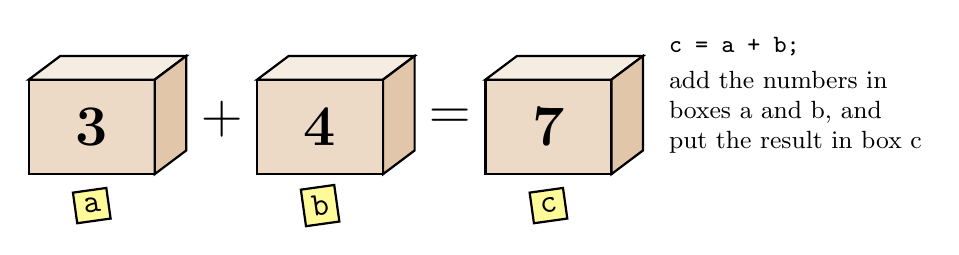
\begin{tikzpicture}[line width=0.8pt]
    \foreach \x/\n/\v in {0/a/3, 2.9/b/4, 5.8/c/7} {
      \filldraw[fill=brown!30]  (\x,0) rectangle +(1.6,1.2);
      \filldraw[fill=brown!15]  (\x,1.2) -- +(0.4,0.3) -- +(2.0,0.3) -- +(1.6,0) -- cycle;
      \filldraw[fill=brown!45]  (\x+1.6,0) -- +(0.4,0.3) -- +(0.4,1.5) -- +(0,1.2) -- cycle;
      \node[font=\huge\bfseries] at (\x+0.8,0.6) {\v};
      \node[draw, fill=yellow!40, rotate=8, font=\ttfamily\large,
            inner sep=3pt] at (\x+0.8,-0.4) {\n};
    }
    \node[font=\huge] at (2.45,0.7) {+};
    \node[font=\huge] at (5.35,0.7) {=};
    \node[font=\small, align=left, anchor=west] at (8.0,1.0)
      {\texttt{c = a + b;}\\[2pt]add the numbers in\\boxes a and b, and\\put the result in box c};
  \end{tikzpicture}
  \caption{Variables are like boxes with labels}
  \label{fig:boxes}
\end{figure}

\texttt{int c;} only gets the box; it puts nothing in it. So what is in \texttt{c} at that point? Nobody knows---it could be any number at all. That is why you must always give a variable a value before you use it.

\texttt{c = a + b;} first takes out the values of \texttt{a} and \texttt{b}, works out $3 + 4 = 7$, and then puts 7 into \texttt{c}. Note that \texttt{=} in C is not the ``equals'' of mathematics. It means ``put in'', and it is called \emph{assignment}.\lazynote{Assignment}{Putting the value worked out on the right of \texttt{=} into the variable on the left. Not the same thing as ``equals'' in mathematics.} So \texttt{a = 10;} throws out the 3 that was in \texttt{a} and puts 10 in its place. In mathematics, this line makes no sense:
\begin{minted}[linenos=false]{c}
x = x + 1;
\end{minted}
In C it is perfectly normal: take out the value of \texttt{x}, add 1, and put it back into \texttt{x}. The result is that \texttt{x} goes up by 1. We will write this a lot.

\texttt{printf} has learned a new trick, too. The \texttt{\%d} in the string is a ``blank'' that means ``an integer goes here''. The values after the string fill these blanks in order: the first \texttt{\%d} gets \texttt{a}, the second gets \texttt{b}, and the third gets \texttt{c}.

Variable names can use English letters, digits and the underscore, but they cannot start with a digit, and they cannot be words that C has already taken, such as \texttt{int} or \texttt{if}. Upper and lower case are different: \texttt{a} and \texttt{A} are two different variables. A good name tells you what is in the box, like \texttt{score} or \texttt{count}.

Besides \texttt{int}, C has other types, such as \texttt{double}, which holds numbers with a decimal point, and \texttt{char}, which holds characters. In this chapter we use only \texttt{int}, and that is already enough to do plenty.

\section{Arithmetic: Making the Program Do Math}
\label{sec:arith}

\codefile{code/en/ch02/arith.c}{Add, subtract, multiply, divide and remainder}{lst:arith}

Output:
\inputminted[linenos=false]{text}{code/en/ch02/out/arith.txt}

Table~\ref{tab:arith} shows the five arithmetic operators of C.

\begin{table}[htbp]
  \centering
  \caption{Arithmetic operators}
  \label{tab:arith}
  \small
  \begin{tabular}{cll}
    \toprule
    Operator & Meaning & Example \\
    \midrule
    \texttt{+} & add & \texttt{17 + 5} gives 22 \\
    \texttt{-} & subtract & \texttt{17 - 5} gives 12 \\
    \texttt{*} & multiply & \texttt{17 * 5} gives 85 \\
    \texttt{/} & divide (for integers, just the quotient) & \texttt{17 / 5} gives 3 \\
    \texttt{\%} & remainder & \texttt{17 \% 5} gives 2 \\
    \bottomrule
  \end{tabular}
\end{table}

Two things need special care:
\begin{itemize}
  \item the multiplication sign is \texttt{*}, not $\times$;
  \item when you divide one integer by another, the result is still an integer,\lazyhint{To get a decimal answer, use the \texttt{double} type, e.g.\ \texttt{17.0 / 5} gives 3.4.} and the fraction is simply thrown away: \texttt{17 / 5} gives 3, not 3.4. If you want to know how much was thrown away, use \texttt{\%} to get the remainder: $17 = 5 \times 3 + 2$, so \texttt{17 \% 5} gives 2.
\end{itemize}

The remainder may not look like much, but it is very useful: if a number divided by 2 leaves 0, the number is even; the remainder of a number of seconds divided by 60 is the seconds left over that don't make a full minute. We will use it in the very next section.

The order of calculation is the same as in mathematics: multiplication and division first, then addition and subtraction, and anything in parentheses before everything else. Because \texttt{\%} has a special meaning inside a \texttt{printf} string, to print a \texttt{\%} you have to write \texttt{\%\%}.

Finally, the boxes have a limited size. An \texttt{int} can hold numbers between about minus 2.1 billion and plus 2.1 billion (to be exact, the largest is 2\,147\,483\,647). A year has 31\,536\,000 seconds, which still fits; the number of seconds in a hundred years does not, and the result would be some strange, meaningless number.

\section{Reading from the Keyboard: \texorpdfstring{\NoCaseChange{scanf}}{scanf}}
\label{sec:scanf}

So far, all the numbers in our programs have been fixed in the code. For a program to interact with people, it has to read what is typed on the keyboard. \texttt{printf} does the ``talking'', and \texttt{scanf} does the ``listening'':

\codefile{code/en/ch02/add.c}{Read two numbers and add them up}{lst:add}

Run it, type \texttt{3 4} and press Enter:
\inputminted[linenos=false]{text}{code/en/ch02/out/add.txt}

\texttt{scanf("\%d \%d", \&a, \&b)} means: read two integers from the keyboard, put the first into \texttt{a} and the second into \texttt{b}. Just as with \texttt{printf}, \texttt{\%d} stands for an integer.

Never forget the \texttt{\&} in front of the variable names.\lazyhint{Forgetting the \texttt{\&} is one of the most common beginner mistakes. Section~\ref{sec:swap} explains why it is needed.} We will explain why it is there when we get to ``pointers''. For now, just remember: \textbf{when you read into a variable with \texttt{scanf}, put \texttt{\&} in front of its name}.

What happens if you don't type numbers---say, you type \texttt{abc}? \texttt{scanf} cannot read an integer, so nothing gets put into \texttt{a} and \texttt{b}. Luckily, \texttt{scanf} tells us how many numbers it managed to read. In the code, \texttt{if (scanf(...) != 2)} means ``if we did not read two numbers'': in that case the program prints a message and ends with \texttt{return 1;}. Returning 1 instead of 0 tells the system that the program did not finish normally. From now on, every program in this chapter checks each call to \texttt{scanf} in this way.

\section{\texorpdfstring{\NoCaseChange{if}}{if} and \texorpdfstring{\NoCaseChange{else}}{else}: Making Decisions}
\label{sec:if}

A program can't always just run from top to bottom; sometimes it has to do different things depending on the situation. For example, deciding whether a number is odd or even:

\codefile{code/en/ch02/even_odd.c}{Odd or even}{lst:even-odd}

\inputminted[linenos=false]{text}{code/en/ch02/out/even_odd.txt}

The parentheses after \texttt{if} contain a \emph{condition}.\lazynote{Condition}{An expression whose result is either ``true'' or ``false''. In C, 0 means false and anything else means true.} \texttt{n \% 2 == 0} asks: ``Is the remainder of \texttt{n} divided by 2 equal to 0?'' If it is, the code in the pair of braces right after it runs; otherwise, the code in the braces after \texttt{else} runs. There are two roads, and only one of them is taken (Figure~\ref{fig:fork}).

\begin{figure}[htbp]
  \centering
  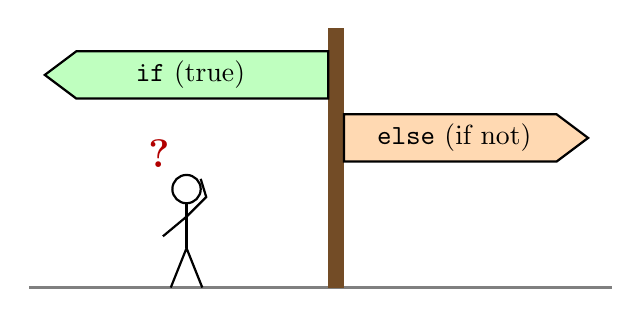
\begin{tikzpicture}[line width=0.8pt]
    \draw[gray, line width=1pt] (-3.8,0) -- (3.6,0);
    \fill[brown!60!black] (0,0) rectangle (0.2,3.3);
    \filldraw[fill=green!25]
      (0,2.4) -- (-3.2,2.4) -- (-3.6,2.7) -- (-3.2,3.0) -- (0,3.0) -- cycle;
    \node at (-1.75,2.7) {\texttt{if} (true)};
    \filldraw[fill=orange!30]
      (0.2,1.6) -- (2.9,1.6) -- (3.3,1.9) -- (2.9,2.2) -- (0.2,2.2) -- cycle;
    \node at (1.6,1.9) {\texttt{else} (if not)};
    % A little person at the fork, scratching their head
    \draw (-1.8,1.25) circle (0.18);
    \draw (-1.8,1.07) -- (-1.8,0.5);
    \draw (-1.8,0.5) -- (-2.0,0) (-1.8,0.5) -- (-1.6,0);
    \draw (-1.8,0.9) -- (-2.1,0.65);
    \draw (-1.8,0.9) -- (-1.55,1.15) -- (-1.62,1.38);
    \node[red!70!black, font=\Large\bfseries] at (-2.15,1.7) {?};
  \end{tikzpicture}
  \caption{The condition decides which road to take}
  \label{fig:fork}
\end{figure}

If there are more than two cases, you can use \texttt{else if} to keep asking, one question after another:

\codefile{code/en/ch02/grade.c}{A comment for every score}{lst:grade}

\inputminted[linenos=false]{text}{code/en/ch02/out/grade.txt}

The program checks the conditions one by one, from top to bottom. As soon as it finds one that is true, it runs that code and doesn't look at the rest. So a score of 95 gets only ``Excellent'', not ``Good'' and ``A pass'' as well. The final \texttt{else} runs only when none of the conditions above it are true.

The code inside the braces is indented four spaces to the right. Indentation makes no difference to how the program runs, but it lets people see at a glance which code belongs to which \texttt{if}. It's a good habit---start it now.

\section{Comparisons and Logic}
\label{sec:logic}

The conditions of \texttt{if} are usually written with the operators in Table~\ref{tab:compare-ops}.

\begin{table}[htbp]
  \centering
  \caption{Comparison and logical operators}
  \label{tab:compare-ops}
  \begin{tabular}{cll}
    \toprule
    Operator & Meaning & Example \\
    \midrule
    \texttt{==} & equal to     & \texttt{n == 5} \\
    \texttt{!=} & not equal to & \texttt{n != 5} \\
    \texttt{<}  & less than    & \texttt{n < 5} \\
    \texttt{>}  & greater than & \texttt{n > 5} \\
    \texttt{<=} & less than or equal to    & \texttt{n <= 5} \\
    \texttt{>=} & greater than or equal to & \texttt{n >= 5} \\
    \midrule
    \texttt{\&\&} & and: both conditions are true     & \texttt{n > 0 \&\& n < 10} \\
    \texttt{||}   & or: at least one is true          & \texttt{n < 0 || n > 10} \\
    \texttt{!}    & not: turns true into false        & \texttt{!(n > 0)} \\
    \bottomrule
  \end{tabular}
\end{table}

With \texttt{\&\&} and \texttt{||} you can combine several conditions. Leap years are a good example: a year is a leap year if it can be divided by 4 but not by 100, or if it can be divided by 400.

\codefile{code/en/ch02/leap.c}{Is it a leap year?}{lst:leap}

\inputminted[linenos=false]{text}{code/en/ch02/out/leap.txt}

To C, ``true'' and ``false'' are really just numbers: a condition that is true gives 1, and one that is false gives 0. The other way round, \texttt{if}, and the \texttt{while} we will meet soon, only check whether the value in the parentheses is 0: 0 counts as false, and anything else counts as true. So \texttt{if (playing)} means ``if \texttt{playing} is not 0''. The game at the end of this chapter uses this.

\begin{quote}
  \textbf{Watch out for \texttt{=} and \texttt{==}!} To test whether two things are equal, use two equals signs. If you write \texttt{if (n = 5)} instead of \texttt{if (n == 5)}, it means ``put 5 into \texttt{n}, then check whether \texttt{n} is 0''---the condition is always true, and the old value of \texttt{n} is gone too. This is one of the most common mistakes in C, and by default \texttt{gcc} doesn't say a word. Compile with the option \texttt{-Wall} (short for ``warn all'', which turns on all the common warnings) and \texttt{gcc} will warn you:
\begin{minted}[linenos=false]{text}
warning: suggest parentheses around assignment used as truth value
\end{minted}
  From now on, it's a good idea to always compile with \texttt{-Wall}: \texttt{gcc -Wall hello.c -o hello}.
\end{quote}

\section{\texorpdfstring{\NoCaseChange{while}}{while} Loops: Doing It Again and Again}
\label{sec:while}

What computers do best is repeat things without ever getting tired. \texttt{while} means ``as long as'': as long as the condition is true, the code in the braces runs again, and again, and again.

\codefile{code/en/ch02/countdown.c}{Rocket countdown}{lst:countdown}

\inputminted[linenos=false, lastline=3]{text}{code/en/ch02/out/countdown.txt}
\vspace{-0.5\baselineskip}
\begin{center}(some lines skipped)\end{center}
\vspace{-0.5\baselineskip}
\inputminted[linenos=false, firstline=10]{text}{code/en/ch02/out/countdown.txt}

\begin{center}
  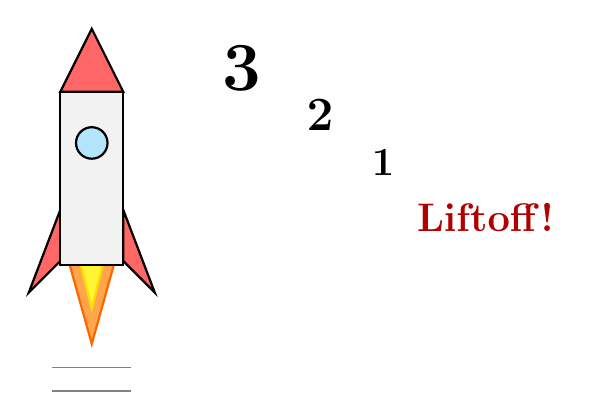
\begin{tikzpicture}[line width=0.8pt]
    \filldraw[fill=orange!70, draw=orange!80!red] (0.12,0) -- (0.4,-1.0) -- (0.68,0) -- cycle;
    \filldraw[fill=yellow!80, draw=yellow!80!orange] (0.26,0) -- (0.4,-0.55) -- (0.54,0) -- cycle;
    \filldraw[fill=red!60] (0,0.05) -- (-0.4,-0.35) -- (0,0.7) -- cycle;
    \filldraw[fill=red!60] (0.8,0.05) -- (1.2,-0.35) -- (0.8,0.7) -- cycle;
    \filldraw[fill=gray!10] (0,0) rectangle (0.8,2.2);
    \filldraw[fill=red!60] (0,2.2) -- (0.4,3.0) -- (0.8,2.2) -- cycle;
    \filldraw[fill=cyan!30] (0.4,1.55) circle (0.2);
    \node[font=\Huge\bfseries]  at (2.3,2.5) {3};
    \node[font=\LARGE\bfseries] at (3.3,1.9) {2};
    \node[font=\Large\bfseries] at (4.1,1.3) {1};
    \node[font=\Large\bfseries, red!70!black] at (5.4,0.6) {Liftoff!};
    \foreach \y in {-1.3,-1.6} \draw[gray, line width=0.6pt] (-0.1,\y) -- (0.9,\y);
  \end{tikzpicture}
\end{center}

This is how the program runs:
\begin{enumerate}
  \item Check the condition \texttt{n > 0}. At first \texttt{n} is 10, so the condition is true.
  \item Run the code in the braces: print \texttt{10...}, then \texttt{n = n - 1}, and \texttt{n} becomes 9.
  \item Go back to step 1 and check the condition again\ldots{}
\end{enumerate}
And so \texttt{n} goes all the way down from 10 to 1. When \texttt{n} becomes 0, the condition is no longer true, the loop ends, and the program goes on to the \texttt{printf("Liftoff!\textbackslash n")} after the loop.

Look at the line \texttt{n = n - 1;} inside the loop. If you forgot it, \texttt{n} would stay 10 forever, the condition would always be true, and the program would print \texttt{10...} on and on without end. This is called an \emph{infinite loop}.\lazynote{Infinite loop}{A loop whose condition is always true, so it never stops. Press \texttt{Ctrl+C} in the terminal to stop the program.} If you ever write one, don't panic: press \texttt{Ctrl+C} in the terminal and the program will stop.

\texttt{while} is best when you don't know in advance how many times something has to be repeated. In a guessing game, for example, nobody knows how many guesses it will take:

\codefile{code/en/ch02/guess.c}{Guess the number}{lst:guess}

\inputminted[linenos=false]{text}{code/en/ch02/out/guess.txt}

As long as \texttt{guess != secret}---that is, as long as the player hasn't got it yet---the program keeps asking for another guess. Each guess adds 1 to \texttt{tries}, and at the end the program tells the player how many guesses it took.

If you always guess right in the middle, you can find any number between 1 and 100 in at most 7 guesses. Can you work out why?

\section{\texorpdfstring{\NoCaseChange{for}}{for} Loops: Repeating While Counting}
\label{sec:for}

There is a story about the German mathematician Gauss. When he was in primary school, his teacher wanted the class to keep quiet for a while and gave them a problem: what is 1 plus 2 plus 3, and so on, all the way up to 100? While the other children were still adding one number at a time, little Gauss quickly put up his hand: $1 + 100 = 101$, $2 + 99 = 101$, \ldots{} there are 50 pairs, so the answer is $50 \times 101 = 5050$.

\begin{center}
  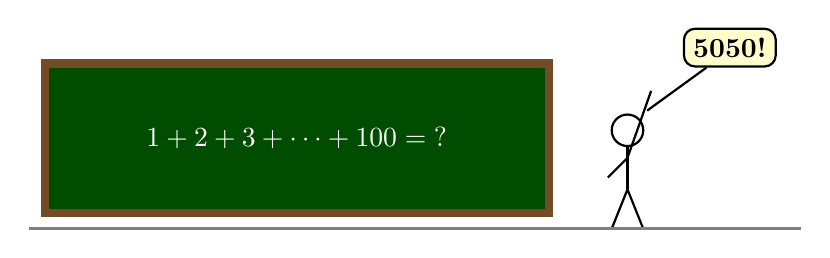
\begin{tikzpicture}[line width=0.8pt]
    \filldraw[fill=green!30!black, draw=brown!60!black, line width=3pt] (0,0) rectangle (6.4,1.9);
    \node[white] at (3.2,0.95) {$1 + 2 + 3 + \cdots + 100 = \;?$};
    % Little Gauss with his hand up
    \draw (7.4,1.05) circle (0.2);
    \draw (7.4,0.85) -- (7.4,0.3);
    \draw (7.4,0.3) -- (7.2,-0.2) (7.4,0.3) -- (7.6,-0.2);
    \draw (7.4,0.7) -- (7.15,0.45);
    \draw (7.4,0.7) -- (7.7,1.55);
    \node[draw, rounded corners, fill=yellow!20, font=\bfseries] (say) at (8.7,2.1) {5050!};
    \draw (say.south west) ++(0.3,0) -- (7.65,1.3);
    \draw[gray, line width=1pt] (-0.2,-0.2) -- (9.6,-0.2);
  \end{tikzpicture}
\end{center}

We are not as clever as Gauss, but we have a computer, and it can patiently add the numbers one at a time:

\codefile{code/en/ch02/sum.c}{Adding up from 0 to 100}{lst:sum}

\inputminted[linenos=false]{text}{code/en/ch02/out/sum.txt}

Same answer as Gauss! For a computer, a hundred additions take no time at all.

The parentheses after \texttt{for} contain three parts, separated by semicolons:
\begin{minted}[linenos=false]{c}
for (i = 0; i <= 100; i++) {
\end{minted}
\begin{enumerate}
  \item \texttt{i = 0}: done once, before anything else, to give the counting variable its starting value;
  \item \texttt{i <= 100}: the condition checked before each round; the loop goes on only if it is true;
  \item \texttt{i++}: done at the end of each round. \texttt{i++} is short for \texttt{i = i + 1}.
\end{enumerate}
So \texttt{i} is 0, 1, 2, \ldots{}, 100 in turn, and each round adds \texttt{i} to \texttt{sum}. In fact, anything a \texttt{for} loop can do, a \texttt{while} loop can do too; but when you are counting ``from here to there'' like this, putting all three parts on one line with \texttt{for} makes it easier to read.

You can also put a loop inside another loop. Remember the triangle in Chapter~\ref{chap:hello} that we wrote out by hand, line by line? Now we can print one as big as we like:

\codefile{code/en/ch02/triangle.c}{A triangle of any size}{lst:triangle}

\inputminted[linenos=false]{text}{code/en/ch02/out/triangle.txt}

The outer \texttt{for} goes down one row at a time; \texttt{row} is the row number. For row number \texttt{row}, the two inner \texttt{for} loops first print \texttt{n - row} spaces, then \texttt{2 * row - 1} stars, and finally a newline. Row 1 has 1 star, row 2 has 3, row 3 has 5\ldots{} and out comes a triangle.

\section{\texorpdfstring{\NoCaseChange{break}}{break}: Leaving a Loop Early}
\label{sec:break}

Sometimes we find what we are looking for before the loop is over. Then we can use \texttt{break} to leave early:

\codefile{code/en/ch02/first_square.c}{The first number whose square is greater than 2000}{lst:first-square}

\inputminted[linenos=false]{text}{code/en/ch02/out/first_square.txt}

\texttt{i} counts up from 1. When it reaches 45, $45 \times 45 = 2025$, which is greater than 2000, so \texttt{break} jumps out of the loop at once, and 46, 47, \ldots{} are never checked. The value left in \texttt{i} is 45.

\texttt{break} only jumps out of the loop it is in. Chapter~\ref{chap:c-structure} shows a clever way to use \texttt{break}.

\section{A Little Game: The Dragon's Cave}
\label{sec:dragon}

By now we can remember things with variables, read the player's choices, make decisions with \texttt{if}, and repeat with loops. That is enough to write a game!

\begin{center}
  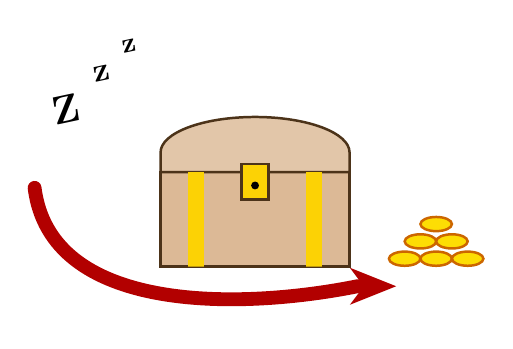
\begin{tikzpicture}[line width=0.9pt]
    % The dragon's tail, curled in front of the chest
    \draw[red!70!black, line width=5pt, line cap=round]
      (-1.6,1.0) .. controls (-1.4,-0.6) and (1.0,-0.55) .. (2.5,-0.25);
    \filldraw[fill=red!70!black, draw=red!70!black]
      (2.45,-0.05) -- (2.95,-0.25) -- (2.45,-0.45) -- (2.6,-0.25) -- cycle;
    % The treasure chest
    \filldraw[fill=brown!55, draw=brown!40!black] (0,0) rectangle (2.4,1.2);
    \filldraw[fill=brown!45, draw=brown!40!black]
      (0,1.2) -- (0,1.45) arc[start angle=180, end angle=0, x radius=1.2, y radius=0.45]
      -- (2.4,1.2) -- cycle;
    \fill[yellow!70!orange] (0.35,0) rectangle (0.55,1.2) (1.85,0) rectangle (2.05,1.2);
    \filldraw[fill=yellow!70!orange, draw=brown!40!black] (1.03,0.85) rectangle (1.37,1.3);
    \fill[black] (1.2,1.03) circle (0.05);
    % Gold coins
    \foreach \x/\y in {3.1/0.1, 3.5/0.1, 3.9/0.1, 3.3/0.32, 3.7/0.32, 3.5/0.54} {
      \filldraw[fill=yellow!80!orange, draw=orange!80!black]
        (\x,\y) ellipse[x radius=0.2, y radius=0.09];
    }
    % Snoring
    \node[font=\Large\bfseries, rotate=12]  at (-1.2,2.0) {Z};
    \node[font=\large\bfseries, rotate=12]  at (-0.75,2.45) {z};
    \node[font=\normalsize\bfseries, rotate=12] at (-0.4,2.8) {z};
  \end{tikzpicture}

  \smallskip
  (Shh---the dragon is snoring.)
\end{center}

\subsection{The Rules}

Legend says a chest of gold is hidden in the dragon's cave in the hills. Torch in hand, you stand at the entrance. There are four places in the cave (Figure~\ref{fig:cave-map}): the entrance, a fork, a small room, and the dragon's lair. The chest is in the lair, and a big red dragon is fast asleep on top of it.

\begin{figure}[htbp]
  \centering
  \begin{tikzpicture}[
      place/.style={draw, rounded corners, fill=brown!10, minimum width=22mm,
                    minimum height=12mm, align=center},
      way/.style={thick, {Stealth}-{Stealth}},
    ]
    \node[place]                     (door)  {Entrance\\\texttt{\small room = 1}};
    \node[place, right=14mm of door] (fork)  {Fork\\\texttt{\small room = 2}};
    \node[place, above right=4mm and 14mm of fork] (small) {Small room\\\texttt{\small room = 3}};
    \node[place, below right=4mm and 14mm of fork, fill=red!10] (lair) {Dragon's lair\\\texttt{\small room = 4}};
    \draw[way] (door) -- (fork);
    \draw[way] (fork) -- node[above left, font=\small] {left} (small);
    \draw[way] (fork) -- node[below left, font=\small] {right} (lair);
    \node[right=2mm of small, font=\small, align=left] {A key hangs\\on the wall};
    \node[right=2mm of lair, font=\small, align=left] {Dragon and\\chest};
  \end{tikzpicture}
  \caption{Map of the dragon's cave}
  \label{fig:cave-map}
\end{figure}

At every step, the game tells you where you are and what you can do, and you type the number of your choice. Be careful: the torch lasts only 12 steps, and once it burns out you can't see a thing. As for how to get the chest\ldots{} try it and find out. A small hint: the dragon seems to like people who are good at math.

\needspace{12\baselineskip}
\subsection{The Program}

\codefile{code/en/ch02/dragon.c}{The Dragon's Cave}{lst:dragon}

\subsection{Let's Play}

\inputminted[linenos=false]{text}{code/en/ch02/out/dragon.txt}

(Spoiler: this is only one way to play. What is the key in the small room for? Find out for yourself.)

\subsection{How the Game Works}

This program is more than a hundred lines long. That looks like a lot, but everything in it is something we have covered in this chapter.

\paragraph{Variables remember the state of the game.} The variables at the start of the program record everything about the game at this moment: \texttt{room} remembers where you are, with 1, 2, 3 and 4 standing for the four places; \texttt{has\_key} remembers whether you have the key, 0 for no and 1 for yes; \texttt{torch} remembers how many more steps the torch will last; and \texttt{playing} remembers whether the game is still going on. Everything that happens in the game world comes down, in the end, to the numbers in these few boxes changing.

\paragraph{One big loop keeps the game going.} \texttt{while (playing)} is the main loop of the whole game. As long as \texttt{playing} is not 0, it goes round and round. Each time round, it does three things:
\begin{enumerate}
  \item \textbf{Describe}: depending on the value of \texttt{room}, use \texttt{if}/\texttt{else if} to print what the place looks like and what you can do there;
  \item \textbf{Read}: read the player's choice with \texttt{scanf}; the torch burns down by one step;
  \item \textbf{Update}: depending on where you are and what you chose, change the values of the variables---change \texttt{room} when you move somewhere else, set \texttt{has\_key} to 1 when you pick up the key, and set \texttt{playing} to 0 when the game is over.
\end{enumerate}
To the player, it feels like ``walking into the cave'' and ``picking up the key''. In the program, that is nothing more than \texttt{room = 2;} and \texttt{has\_key = 1;}.

\paragraph{The dragon's riddle.} The dragon asks exactly the question we worked out in the section on \texttt{for} loops. A \texttt{for} loop gives the player 3 tries; a right answer leaves the loop early with \texttt{break} and sets \texttt{won} to 1. After the loop, if \texttt{won} is still 0, all 3 answers were wrong.

This ``describe--read--update'' loop is called a \emph{game loop}.\lazynote{Game loop}{Describe, read, update, round and round. Almost every game is built this way.} From the simplest text game to big games with beautiful graphics, they are all built this way---big games just go round the loop dozens of times a second. Remember the CPU at the end of Chapter~\ref{chap:hello}? It, too, runs a loop that never stops: fetch, decode, execute, write back. It seems loops really are the heartbeat of the computer world.

\subsection{Make It Your Own}

The game is yours now. Change whatever you like:
\begin{itemize}
  \item make the torch last only 8 steps, and see if you can still get the chest;
  \item change the riddle, for example to ``what is 1 plus 2 plus \ldots{} plus 1000?'', or have the dragon ask for your birthday;
  \item add a new place, such as an underground river behind the small room. Give it a new \texttt{room} number, and add an \texttt{else if} to both the ``describe'' part and the ``update'' part;
  \item add a new item, such as a sword. Use a new variable, \texttt{has\_sword}, to remember whether you have it.
\end{itemize}
When you are done, run \texttt{make test} to see whether the original ways of playing still work. If you changed the rules of the game, it's normal for the tests to report \texttt{FAIL}---that just shows they are checking carefully.

\section{Summary}

\begin{itemize}
  \item A variable is a box with a label. An \texttt{int} variable holds an integer; \texttt{=} is assignment, which puts the value on the right into the variable on the left.
  \item The arithmetic operators are \texttt{+ - * / \%}. Dividing one integer by another gives just the quotient; \texttt{\%} gives the remainder.
  \item \texttt{printf} prints an integer with \texttt{\%d}; \texttt{scanf} reads one with \texttt{\%d}, with \texttt{\&} in front of the variable name.
  \item \texttt{if}/\texttt{else if}/\texttt{else} choose which code to run based on conditions. Test for equality with \texttt{==}, not \texttt{=}; compile with \texttt{-Wall}.
  \item \texttt{\&\&}, \texttt{||} and \texttt{!} combine conditions. In C, 0 means false and anything else means true.
  \item \texttt{while} repeats as long as its condition is true; \texttt{for} is good for counting ``from here to there''; \texttt{break} leaves a loop early. Stop an infinite loop with \texttt{Ctrl+C}.
  \item A game uses variables to remember its state, and goes round a loop: describe, read, update.
\end{itemize}

\section*{Exercises}

\begin{enumerate}
  \item Write a program that reads a number of seconds, such as 3725, and prints how many hours, minutes and seconds that is (1 hour, 2 minutes and 5 seconds). Hint: use \texttt{/} and \texttt{\%}.
  \item Change Listing~\ref{lst:sum} to add up all the even numbers from 1 to 100. (The answer is 2550.)
  \item Use \texttt{for} loops to print a multiplication table from $1 \times 1$ up to $9 \times 9$.
  \item Change Listing~\ref{lst:guess} so that if the player still hasn't got it after 7 guesses, the program tells them the answer and the game ends.
  \item Change Listing~\ref{lst:triangle} to print an upside-down triangle.
  \item Add a new place and a new item to the Dragon's Cave, then write a test for them and add it to \texttt{test.sh}.
\end{enumerate}
